\documentclass[dvipdfmx,12pt]{beamer}% dvipdfmxしたい
\usepackage{bxdpx-beamer}% dvipdfmxなので必要
\usepackage{pxjahyper}% 日本語で'しおり'したい
\usepackage{minijs}% min10ヤダ
\usepackage{amsmath,amssymb,amsthm}% 数式とか
\usepackage{graphicx}% 画像とか
\usepackage{tikz}% 図とか
\usepackage{ascmac}% 枠とか
\usepackage{url}% URLとか
\usepackage{here}% 画像とか
\usepackage{hyperref}% ハイパーリンクとか
\renewcommand{\kanjifamilydefault}{\gtdefault}% 既定をゴシック体に

% あとは欧文の場合と同じ
\usetheme{Copenhagen}% https://hartwork.org/beamer-theme-matrix/
\usecolortheme{default}% https://hartwork.org/beamer-theme-matrix/

\AtBeginSection[]{
    \frame{\tableofcontents[currentsection, hideallsubsections]} %目次スライド
}

\title{今週のAINews}
\author{中園康聖}
\date{2024/03/06}
\setbeamertemplate{caption}[numbered]
\begin{document}
\bibliographystyle{junsrt}% 参考文献のスタイル(https://mathlandscape.com/latex-bibstyles/)
\begin{frame}
\titlepage
\end{frame}
\begin{frame}{目次}
\tableofcontents
\end{frame}
\section{OpenAIとロボット}
\subsection{FigureAI}
\begin{frame}
\frametitle{FigureAI、OpenAIから資金提供を受ける}

FigureAIが、MicrosoftやNvidia、OpenAIなどから6億7500万ドル(約1000億円)の資金提供を受けた。
FigureAIは、人型ロボットの開発を行っており、今後はOpenAIとの協力を強化するとしている。以下はデモ動画である。
\begin{itemize}
\item \href{https://www.youtube.com/watch?v=-4erYt2t7Bs}{2足歩行}
\item \href{https://www.youtube.com/watch?v=Q5MKo7Idsok}{コーヒーを淹れる}
\item \href{https://www.youtube.com/watch?v=gEjXcEU3BbwURL}{物を運ぶ}
\item \href{https://www.youtube.com/watch?v=Sq1QZB5baNw}{人と対話する(OpenAIと連携)}
\item \href{https://twitter.com/ctgptlb/status/1767919292836945922?s=12&t=HWsH9aiIPwtM8W1pjX9WBA}{日本語字幕付き}
\end{itemize}
\end{frame}

\subsection{LLMを利用した報酬関数設定「Eureka」}
\begin{frame}
\frametitle{Eureka}
ペン回しのような、低レベルかつ複雑なタスクにLLMを利用することは困難な問題として知られている。
そこで、LLMのコード生成を用いて進化的最適化を行い、報酬関数設計を行う。説明ページは\href{https://eureka-research.github.io/}{こちら}。
\end{frame}

\begin{frame}
\frametitle{Eurekaの構成図}
Eurekaの構成は図\ref{fig:eureka}のようになった。

\begin{figure}[t]
\centering
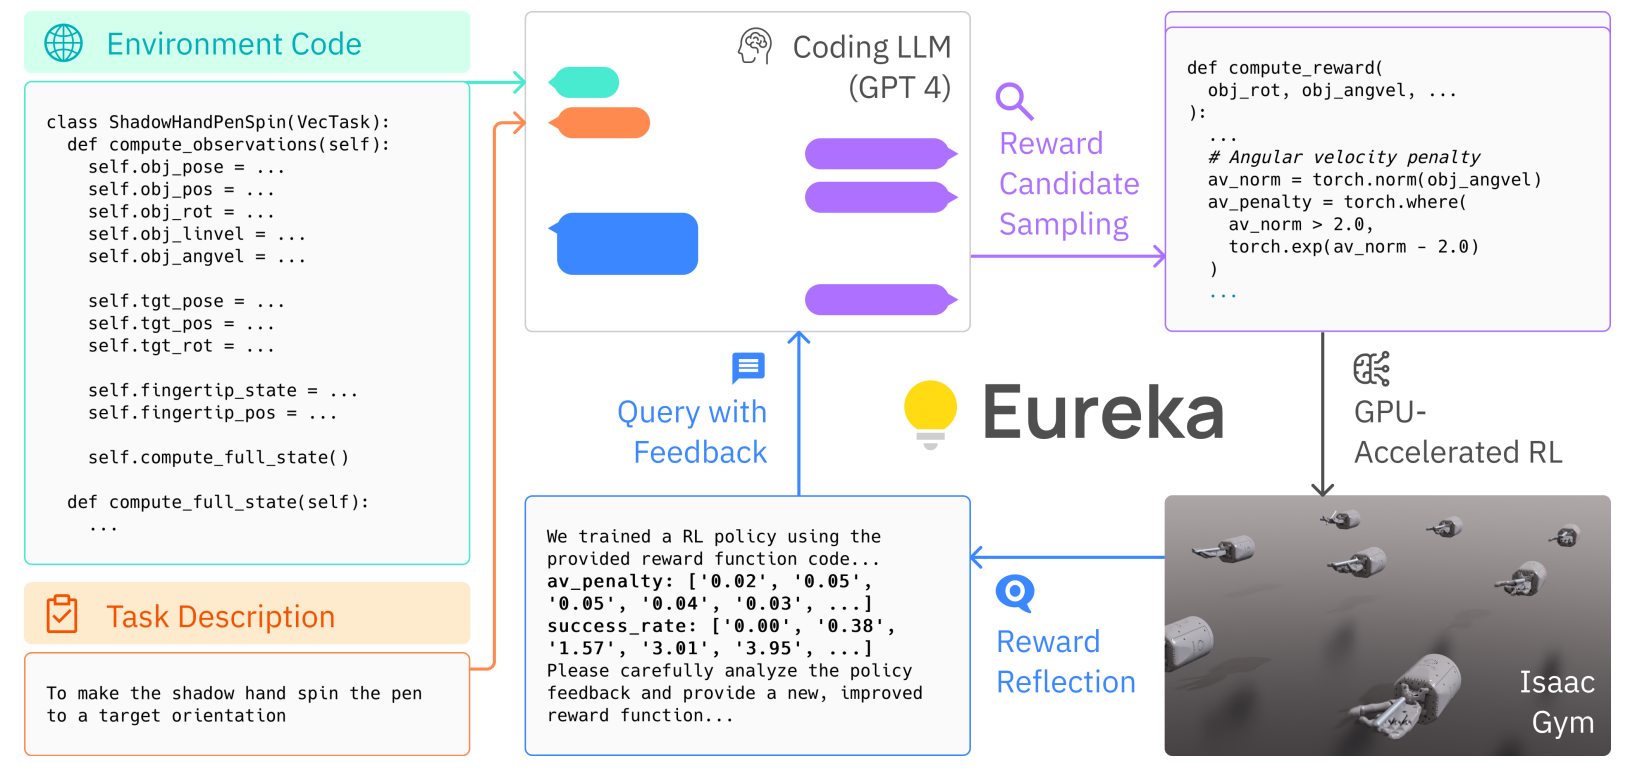
\includegraphics[width=0.8\linewidth]{eureka.png}
\caption{Eurekaの構成図}
\label{fig:eureka}
\end{figure}
\end{frame}

\begin{frame}
\frametitle{結果}
\begin{itemize}
\item 83\%のタスクで、人間が設計した報酬関数よりも良い報酬関数を設計できた。
\item Eurekaは、複雑なタスクほど人の報酬と負の相関を持ったが、いくつかのタスクでは負の相関を持ちながら人間の報酬を上回った。
\end{itemize}
\end{frame}

% \begin{frame}[allowframebreaks]
% \bibliography{sample} %参考文献ファイル名(sample.bib) 拡張子は指定しない
% \end{frame}
\end{document}